\documentclass[12pt]{article}
\usepackage{amsmath,amssymb}

% -- Page Margin --
\usepackage[margin=1in]{geometry}

% -- Imagenes --
\usepackage{graphicx}
\usepackage{float}

% -- Color --
\usepackage{xcolor}
\definecolor{azul}{RGB}{35,72,180}

% -- Espaciados --
\newcommand{\Pspace}{0.5cm}
\newcommand{\Aspace}{0.2cm}

% -- Assets para figura 2.1 --
\newcommand{\lheight}{1.3em}
\newcommand{\lraise}{-0.4em}
\newcommand{\lon}{\raisebox{\lraise}{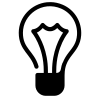
\includegraphics[height=\lheight]{./img/light_on_icon.png}}}
\newcommand{\loff}{\raisebox{\lraise}{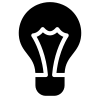
\includegraphics[height=\lheight]{./img/light_off_icon.png}}}

\title
{
    Teoría de la Computación 2026-1 \\
}

    \begin{document}

    \maketitle

    \begin{center}
        \begin{tabular}{r|l}
            \textbf{Expediente} & \textbf{Nombre} \\\hline \vspace{-0.4cm} \\
            223209096 & Ahumada Herrera Jorge Alán \\
            219208106 & Bórquez Guerrero Angel Fernando \\
            222206586 & Juan Valenzuela Gael \\
            223201053 & Solis Zatarain Owen Adiel \\
        \end{tabular}
    \end{center}

    \rule{\linewidth}{0.3mm}

    \vspace{0.3cm}



{ \large \textbf{Ejercicio 92.} } Diseñe dos AP diferentes que acepten por pila vacía al lenguaje aceptado por el AFD de <<los tres focos>> descrito enla figura 2.1.
\renewcommand{\thefigure}{2.\arabic{figure}}
\setcounter{figure}{0}
\begin{figure}[!ht]
\centering
\begin{tabular}{r|ccc}
    & $a$ & $b$ & $c$ \\
    \hline
    \vspace{-0.3cm} \\
    { \large $\rightarrow$ } \hspace{-0.4cm} \loff \loff \loff & \lon \loff \loff & \loff \lon \loff & \loff \loff \lon \\ \vspace{-0.3cm} \\
    
    \lon \loff \loff & \loff \loff \loff & \lon \lon \loff & \lon \loff \lon \\ \vspace{-0.3cm} \\
    
    \loff \lon \loff & \lon \lon \loff & \loff \loff \loff & \loff \lon \lon \\ \vspace{-0.3cm} \\

    \loff \loff \lon & \lon \loff \lon & \loff \lon \lon & \loff \loff \loff \\ \vspace{-0.3cm} \\

    \lon \lon \loff & \loff \lon \loff & \lon \loff \loff & \lon \lon \lon \\ \vspace{-0.3cm} \\

    \lon \loff \lon & \loff \loff \lon & \lon \lon \lon & \lon \loff \loff \\ \vspace{-0.3cm} \\

    { \large $\ast$} \hspace{-0.3cm} \lon \lon \lon & \loff \lon \lon & \lon \loff \lon & \lon \lon \loff \\ \vspace{-0.3cm} \\

    \loff \lon \lon & \lon \lon \lon & \loff \loff \lon & \loff \lon \loff
\end{tabular} 
\caption{Tabla de transición del autómata de los tres focos.}
\end{figure}
\renewcommand{\thefigure}{\arabic{figure}}
    % Respuesta:
    \vspace{\Aspace} \par
    { \color{azul}
        \textbf{Observación previa} \\
        El autómata de los tres focos acepta las cadenas en $\{ a, b, c \}^{*}$ tales que cada foco termina encendido. 
        Esto ocurre si y solo si cada símbolo aparece un número impar de veces. \\
        $L = \{ w \in \{ a, b, c \}^{*}: |w|_{a}, |w|_{b}, |w|_{c} son impares \}$ \\
        Este es un lenguaje regular, por lo que puede ser reconocido por un AP que simule al AFD. \\

        \newpage
        \textbf{Primer AP} \\
        Definimos el AP: \\
        $M_{1} = (Q, \Sigma, \Gamma, \delta, q_{0}, Z_{0})$ \\
        donde: 
        \begin{itemize}
            \item $Q = \{ q_{000}, q_{100}, q_{010}, q_{001}, q_{110}, q_{101}, q_{011}, q_{111} \}$

            \item $\Sigma = \{ a, b, c \}$

            \item $\Gamma = \{ Z_0 \}$

            \item Estado inicial: $q_{000}$
        \end{itemize}
        Cada estado representa la paridad de ($a$, $b$, $c$). \\
        La pila nunca cambia (solo contiene $Z_{0}$). \\
        Las transiciones son: \\
        $\delta(q, x, Z_{0}) = (q', Z_{0})$ \\
        donde $q'$ cambia la paridad correspondiente. \\

        Por ejemplo: \\
        $\delta(q_{000}, a, Z_{0}) = (q_{100}, Z_{0})$ \\
        $\delta(q_{100}, a, Z_{0}) = (q_{000}, Z_{0})$ \\
        y análogamente para $b$ y $c$. \\

        Finalmente, se vacía la pila si se llega a $q_{111}$: \\
        $\delta (q_{111}, \varepsilon, Z_{0}) = (q_{111}, \varepsilon)$ \\
        Por tanto, acepta por pila vacía. \\

        \vspace{\Pspace}

        \textbf{Segundo AP} \\
        Construimos un AP distinto usando conteo en pila. \\
        $M_2 = (Q, \Sigma, \Gamma, \delta, q_0, Z_{0})$ \\
        donde:
        \begin{itemize}
            \item $Q = \{ q \}$

            \item $\Sigma = \{ a, b, c \}$

            \item $\Gamma = \{ A, B, C, Z_{0} \}$
        \end{itemize}
        
        La idea es:
        \begin{itemize}
            \item Cada vez que aparece $a$, alternamos entre empujar y sacar $A$.

            \item Igual para $b$ y $c$.
        \end{itemize}

        \newpage
        Ejemplo para $a$: \\
        $\delta (q, a, Z_{0}) = (q, AZ_0)$ \\
        $\delta (q, a, A) = (q, \varepsilon)$ \\

        Análogamente para $B$ y $C$. \\
        Al final, la pila queda vacía si cada símbolo apareció un número par de veces de empuje/salida,
        lo que corresponde a impar en total (por construcción alternada). \\
        Finalmente: \\
        $\delta (q, \varepsilon, Z_0) = (q, \varepsilon)$ \\
        Este AP es distinto porque usa la pila activamente.
    }



% ---------------------------------------------------------------------------



\newpage { \large \textbf{Ejercicio 106.} } Pruebe que $A \overset{*}{\Rightarrow} \gamma$ si y solo si cualesquiera $\alpha$, $\beta \in (T \cup V)^{*}$,
$\alpha A \beta \overset{*}{\Rightarrow} \alpha \gamma \beta$. Encuentre un contraejemplo para demostrar que en general no es cierto que si 
$\alpha A \beta \overset{*}{\Rightarrow} \alpha \gamma \beta$ para algunas cadenas $\alpha$ y $\beta$ entonces $A \overset{*}{\Rightarrow} \gamma$.
    % Respuesta:
    \vspace{\Aspace} \par
    { \color{azul} 
        \textbf{Demostración} \\
        ($\Rightarrow$) Suponga $A \equiv \gamma$ \\
        Por definición de equivalencia en gramáticas, $A$ puede ser reemplazado por $\gamma$ en cualquier contexto \\
        Por tanto, para cualesquiera $\alpha$, $\beta$: \\
        $\alpha A \beta \Rightarrow \alpha \gamma \beta$ \\

        \hspace{-0.6cm}($\Leftarrow$) Suponga que: \\
        $\forall \alpha$, $\beta$, $\alpha A \beta \Rightarrow \alpha \gamma \beta$ \\
        Tomando $\alpha = \varepsilon$ y $\beta = \varepsilon$: \\
        $A \Rightarrow \gamma$ \\

        Además, como la sustitución es válida en cualquier contexto, implica equivalencia estructural, por lo que: \\
        $A \equiv \gamma$ \\ \\

        \textbf{Contraejemplo} \\
        Sea la gramática: \\
        $A \rightarrow a | b$ \\
        y $\gamma = a$ \\
        Entonces: \\
        $A \Rightarrow a$ \\
        pero también: \\
        $A \Rightarrow b$ \\

        Ahora, para algunas cadenas (por ejemplo con $\alpha = \varepsilon$, $\beta = \varepsilon$): \\
        $A = a$ \\
        pero no es cierto que: \\
        $A \equiv a$ \\
        porque $A$ geneara más cadenas. \\

        Esto demuestra que no basta que la propiedad se cumpla para algunas $\alpha$, $\beta$. \\ \\

        \textbf{Conclusión} \\
        Se construyeron dos AP distintos que aceptan el mismo lenguaje (uno simulando el AFD y el otro usando la pila activamente),
        y se probó formalmente la equivalenica del ejercicio 106 junto con un contraejemplo que muestra la necesidad de la condición universal.
    }




% ---------------------------------------------------------------------------



\newpage { \large \textbf{Ejercicio 109.} } Una \textit{gramática regular} (por la derecha) es una GLC que admite solo producciones de la forma: \par
$A \rightarrow aB$ \par
$C \rightarrow b$ \par
$D \rightarrow \varepsilon$ \par
donde $A$, $B$, $C$, $D$ son variables sintácticas y $a$, $b$ son símbolos terminales.
Encuentre una gramática regular para los siguientes conjuntos:
\begin{enumerate}
    \item El conjunto de cadenas binarias que terminan en 111.
        % Respuesta:
        \vspace{\Aspace} \par
        { \color{azul}
            \textbf{Gramática regular} \\
            Cada variable rastrea cuántos 1s consecutivos lleva la cadena al final: \\
            $S$: cero, $A$: uno, $B$: dos, $C$: tres o más. \\

            Definimos $G = (V, T, P, S)$ con $V = \{ S, A, B, C \}$, $T = \{ 0, 1 \}$. \\
            Producciones $P$: \\
            \begin{tabular}{ccccccc}
                $S$ & $\rightarrow$ & $0S$ & | & $1A$ && \\
                $A$ & $\rightarrow$ & $0S$ & | & $1B$ && \\
                $B$ & $\rightarrow$ & $0S$ & | & $1C$ && \\
                $C$ & $\rightarrow$ & $0S$ & | & $1C$ & | & $\varepsilon$ \\
            \end{tabular} \\

            \textbf{Verificaci\'on:} \\
            $S \Rightarrow 1A \Rightarrow 11B \Rightarrow 111C \Rightarrow 111$ \quad (acepta ``111'') \\
            $S \Rightarrow 0S \Rightarrow 01A \Rightarrow 011B \Rightarrow 0111C \Rightarrow 0111$ \quad (acepta ``0111'') \\
            $S \Rightarrow 1A \Rightarrow 11B \Rightarrow 110S$ \quad ($S$ no deriva $\varepsilon$, rechaza ``110'')
        }


    \item $L_{a} = \{a^{2m + 1}: m \geq 0\}$.
        % Respuesta:
        \vspace{\Aspace} \par
        { \color{azul} 
            \textbf{Gramática regular} \\
            Este lenguaje es el conjunto de cadenas con cantidad impar de $a$: $\{ a, aaa, aaaaa, \ldots \}$. \\
            Dos variables que alternan la paridad. \\

            Definimos $G = (V, T, P, S)$ con $V = \{ S, A \}$, $T = \{ a \}$. \\
            Producciones $P$: \\
            \begin{tabular}{ccc}
                $S$ & $\rightarrow$ & $aA$ \\
                $A$ & $\rightarrow$ & $aS$ \\
                & | & $\varepsilon$
            \end{tabular} \\

            $S$ = cantidad par de $a$ le\'idas (inicio, 0 es par). \\
            $A$ = cantidad impar de $a$ le\'idas (puede derivar $\varepsilon$). \\ 

            \textbf{Verificación:} \\
            $S \Rightarrow aA \Rightarrow a$ \quad (acepta $a$, $m = 0$) \\
            $S \Rightarrow aA \Rightarrow aaS \Rightarrow aaaA \Rightarrow aaa$ \quad (acepta $aaa$, $m = 1$) \\
            $S \Rightarrow aA \Rightarrow aaS$ \quad ($S$ no deriva $\varepsilon$, rechaza $aa$)
        }


    \item El conjunto de cadenas binarias con una cantidad impar de ceros y una cantidad impar de unos.
        % Respuesta:
        \vspace{\Aspace} \par
        { \color{azul}
            \textbf{Gramática regular} \\
            Rastreamos la paridad de ambos símbolos simultáneamente ($2 \times 2 = 4$ combinaciones).

            Definimos $G = (V, T, P, S)$ con $V = \{ S, A, B, C \}$, $T = \{ 0, 1 \}$.
            \vspace{-0.2cm}
            \begin{itemize}
                \item $S$: par de 0s, par de 1s (inicio).
                \item $A$: impar de 0s, par de 1s.
                \item $B$: par de 0s, impar de 1s.
                \item $C$: impar de 0s, impar de 1s (\textbf{aceptor}, deriva $\varepsilon$).
            \end{itemize}
            Producciones $P$: \\
            \begin{tabular}{ccc}
                $S$ & $\rightarrow$ & $0A$ \\
                & | & $1B$ \\
                $A$ & $\rightarrow$ & $0S$ \\
                & | & $1C$ \\
                $B$ & $\rightarrow$ & $0C$ \\
                & | & $1S$ \\
                $C$ & $\rightarrow$ & $0B$ \\
                & | & $1A$ \\
                & | & $\varepsilon$ \\
            \end{tabular} \\

            Cada $0$ cambia la paridad de los ceros; cada $1$ cambia la paridad de los unos. \\
            Solo $C$ puede derivar $\varepsilon$ (ambas paridades impares). \\

            \textbf{Verificación:} \\
            $S \Rightarrow 0A \Rightarrow 01C \Rightarrow 01$ \quad (acepta ``01'': 1 cero, 1 uno) \\
            $S \Rightarrow 1B \Rightarrow 10C \Rightarrow 10$ \quad (acepta ``10'': 1 cero, 1 uno) \\
            $S \Rightarrow 0A \Rightarrow 00S \Rightarrow 001B \Rightarrow 0011S$ \quad ($S$ no deriva $\varepsilon$, rechaza ``0011'')
        }

    
    \newpage
    \item $L_{\text{son}}$ el lenguaje del ejemplo 15.
    \renewcommand{\thefigure}{2.\arabic{figure}}
    \setcounter{figure}{4}
    \begin{figure}[!ht]
        \centering
        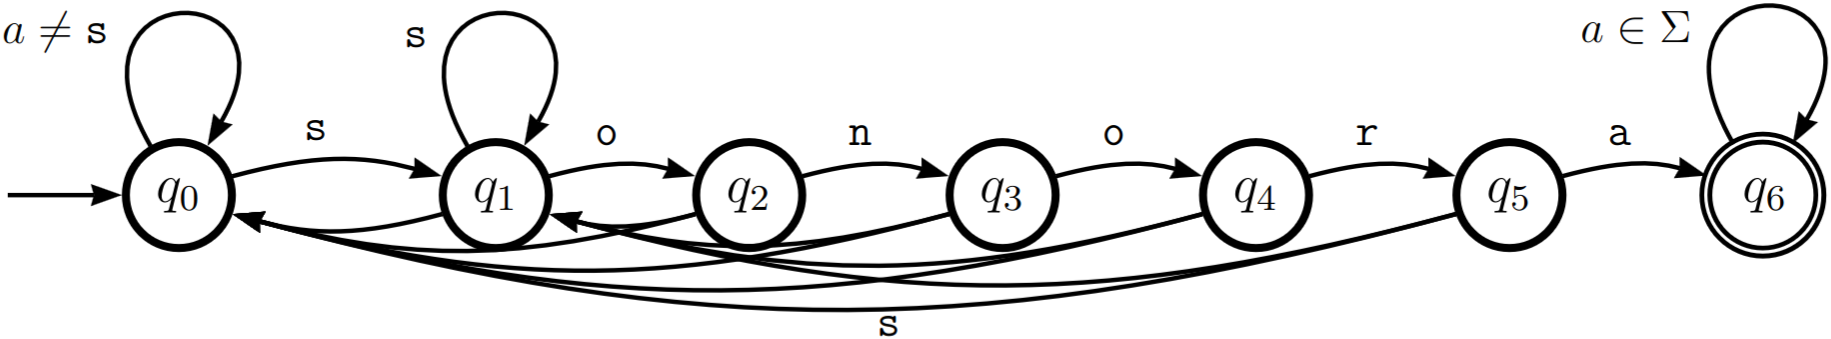
\includegraphics[width=0.8\textwidth]{./img/figura_2.3.png}
        \caption{Autómata que lee \texttt{sonora}.}
    \end{figure}
    \renewcommand{\thefigure}{\arabic{figure}}
        % Respuesta:
        \vspace{\Aspace} \par
        { \color{azul}
            \textbf{Gramática regular} \\
            Cada estado del AFD se convierte en una variable. \\
            Definimos $G = (V, \Sigma, P, S)$ con $V = \{ S, A, B, C, D, E, F \}$, $\Sigma = \{ s, o, n, r, a \}$.
            \vspace{-0.2cm}
            \begin{itemize}
                \item $S$ ($q_0$): sin progreso (inicio).
                \item $A$ ($q_1$): le\'ido \textbf{s}.
                \item $B$ ($q_2$): le\'ido \textbf{so}.
                \item $C$ ($q_3$): le\'ido \textbf{son}.
                \item $D$ ($q_4$): le\'ido \textbf{sono}.
                \item $E$ ($q_5$): le\'ido \textbf{sonor}.
                \item $F$ ($q_6$): le\'ido \textbf{sonora} (\textbf{aceptor}, deriva $\varepsilon$).
            \end{itemize}
            Producciones $P$: \\
            \begin{tabular}{ccccccccccccc}
                $S$ & $\rightarrow$ & $sA$ & | & $oS$ & | & $nS$ & | & $rS$ & | & $aS$ && \\
                $A$ & $\rightarrow$ & $oB$ & | & $sA$ & | & $nS$ & | & $rS$ & | & $aS$ && \\
                $B$ & $\rightarrow$ & $nC$ & | & $sA$ & | & $oS$ & | & $rS$ & | & $aS$ && \\
                $C$ & $\rightarrow$ & $oD$ & | & $sA$ & | & $nS$ & | & $rS$ & | & $aS$ && \\
                $D$ & $\rightarrow$ & $rE$ & | & $sA$ & | & $oS$ & | & $nS$ & | & $aS$ && \\
                $E$ & $\rightarrow$ & $aF$ & | & $sA$ & | & $oS$ & | & $nS$ & | & $rS$ && \\
                $F$ & $\rightarrow$ & $sF$ & | & $oF$ & | & $nF$ & | & $rF$ & | & $aF$ & | & $\varepsilon$ \\
            \end{tabular} \\

            La primera producción de cada variable avanza en la lectura de ``sonora''. \\
            Leer $s$ siempre lleva a $A$ (posible inicio de nuevo ``sonora''). \\
            Cualquier otra letra no esperada regresa a $S$. \\
            $F$ se queda en $F$ con todo s\'imbolo y puede derivar $\varepsilon$. \\

            \textbf{Verificación:} \\
            $S \Rightarrow sA \Rightarrow soB \Rightarrow sonC \Rightarrow sonoD \Rightarrow sonorE \Rightarrow sonoraF \Rightarrow sonora$ \\
            (acepta ``sonora'') \\
            $S \Rightarrow sA \Rightarrow ssA \Rightarrow ssoB \Rightarrow ssonC \Rightarrow ssonoD \Rightarrow ssonorE \Rightarrow ssonoraF \Rightarrow ssonora$ \\
            (acepta ``ssonora'') \\
            $S \Rightarrow sA \Rightarrow soB \Rightarrow sonC$ \quad ($C$ no deriva $\varepsilon$, rechaza ``son'')
        }
\end{enumerate}



% ---------------------------------------------------------------------------



\newpage { \large \textbf{Ejercicio 116.} } Desambigüe la GLC con producciones: \par
\begin{tabular}{ccc}
    $S$ & $\rightarrow$ & $[S]$ \\
    & | & $(S)$ \\
    & | & $\{S\}$ \\
    & | & $SS$ \\
    & | & $\varepsilon$
\end{tabular} \\
    % Respuesta:
    \vspace{\Aspace} \par
    { \color{azul}
    \raggedright
        \textbf{Gramática desambiguada} \\
        Para eliminar la ambigüedad, separamos la gramática en dos niveles: uno que genera un único bloque balanceado ($T$) y otro que genera una secuencia de dichos bloques ($S$). \\

        \vspace{0.5cm}
        Definimos $G = (V, \Sigma, P, S)$ con $V = \{ S, T \}$ y $\Sigma = \{ (, ), [, ], \{, \} \}$. \\
        Producciones $P$: \\
        \begin{tabular}{ccl}
            $S$ & $\rightarrow$ & $T S$ \\
            & | & $\varepsilon$ \\
            $T$ & $\rightarrow$ & $(S)$ \\
            & | & $[S]$ \\
            & | & $\{S\}$ \\
        \end{tabular} \\
        
        \vspace{0.5cm}
        Ya no es posible elegir arbitrariamente dónde "romper" la cadena $SS$. \\
        La cadena vacía $\varepsilon$ solo es generada por $S$, evitando que $T$ pueda ser invisible y crear derivaciones redundantes. \\ 

        \vspace{0.5cm}
        \textbf{Verificación:} \\
        Para la cadena $()()$, la única derivación por la izquierda posible es: \\
        $S \Rightarrow TS \Rightarrow (S)S \Rightarrow (\varepsilon)S \Rightarrow ()TS \Rightarrow ()(S)S \Rightarrow ()(\varepsilon)S \Rightarrow ()()\varepsilon \Rightarrow ()()$ \\
        No existe otra secuencia de reglas que produzca la misma cadena, por lo tanto, la gramática no es ambigua.
    }



% ---------------------------------------------------------------------------



\newpage { \large \textbf{Ejercicio 117.} } La GLC del ejemplo 54 es ambigua.
De dos ejemplos de árboles de derivación para una misma cadena. \\
\textbf{Ejemplo 54}: \\
\begin{tabular}{ccl}
    $S$ & $\rightarrow$ & \texttt{IF} $C$ \texttt{THEN} $S$ \\
    & | & \texttt{IF} $C$ \texttt{THEN} $S$ \texttt{ELSE} $S$ \\
    & | & $E$ \\

    $E$ & $\rightarrow$ & \texttt{print .°k"} \\
    & | & \texttt{break} \\
    & | & \texttt{return true} \\
    & | & \texttt{return false} \\
    & | & $E$, $E$ \\

    $C$ & $\rightarrow$ & \texttt{false} \\
    & | & \texttt{true} \\
\end{tabular}
    % Respuesta:
    \vspace{\Aspace} \par
    { \color{azul} 
        \raggedright
        Cadena: \texttt{IF true THEN IF true THEN break ELSE return true} \\
        \textbf{Ejemplo 1} \\
        \begin{figure}[!ht]
            \centering
            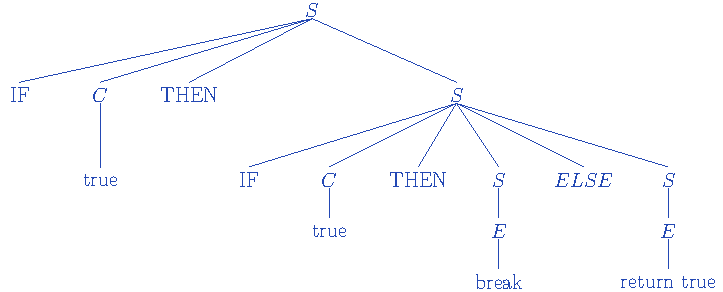
\includegraphics[width=0.9\textwidth]{./figuras/117_a_1/117_a_1.pdf}
        \end{figure} \par

        \textbf{Ejemplo 2} \\
        \begin{figure}[!ht]
            \centering
            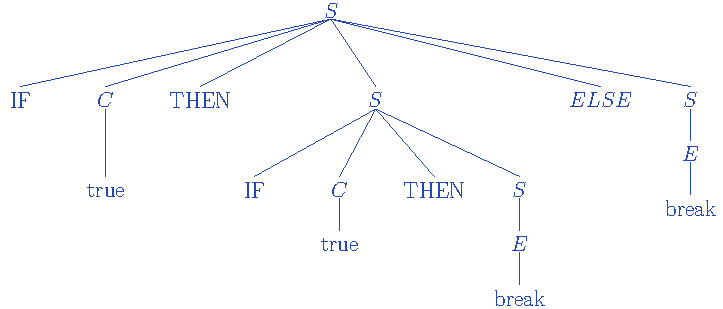
\includegraphics[width=0.9\textwidth]{./figuras/117_a_2/117_a_2.pdf}
        \end{figure}
    }

\newpage
Decide si la siguiente gramática alternativa es ambigua o no: \par
\begin{tabular}{ccl}
    $S$ & $\rightarrow$ & \texttt{IF} $C$ \texttt{THEN} $S$ \texttt{ENDIF} \\
    & | & \texttt{IF} $C$ \texttt{THEN} $S$ \texttt{ELSE} $S$ \texttt{ENDIF} \\
    & | & $E$ \\

    $E$ & $\rightarrow$ & \texttt{print .°k"} \\
    & | & \texttt{break} \\
    & | & \texttt{return true} \\
    & | & \texttt{return false} \\
    & | & $E$ \texttt{print .°k"} \\
    & | & $E$ \texttt{break} \\
    & | & $E$ \texttt{return true} \\
    & | & $E$ \texttt{return false} \\

    $C$ & $\rightarrow$ & \texttt{false} \\
    & | & \texttt{true} \\
\end{tabular} \\
    % Respuesta:
    \vspace{\Aspace} \par
    { \color{azul}
        \raggedright
        La gramática alternativa \textbf{no es ambigua}. \\[6pt]
        La ambigüedad original del Ejemplo 54 se debía al problema de la cadena
        \texttt{IF true THEN IF true THEN break ELSE return true}
        admitía dos árboles de derivación distintos porque no había forma
        de determinar a cuál \texttt{IF} pertenecía el \texttt{ELSE}. \\[6pt]
        En la gramática alternativa, la introducción del token \texttt{ENDIF}
        como marcador de cierre obligatorio resuelve el problema. Ahora las
        dos lecturas antes ambiguas producen cadenas \textbf{distintas}:
        
        \begin{itemize}
            \item \texttt{IF true THEN IF true THEN break ELSE return true
                ENDIF ENDIF} \\
                (el \texttt{ELSE} pertenece al \texttt{IF} interior,
                que cierra con su propio \texttt{ENDIF})
            \item \texttt{IF true THEN IF true THEN break ENDIF ELSE
                return true ENDIF} \\
                (el \texttt{ELSE} pertenece al \texttt{IF} exterior,
                pues el \texttt{IF} interior ya cerró con \texttt{ENDIF})
        \end{itemize}
        Al ser cadenas distintas, ninguna admite dos árboles de derivación.
        En general, dado cualquier \texttt{IF}, el \texttt{ENDIF}
        correspondiente lo cierra de forma unívoca: si aparece \texttt{ELSE}
        antes del \texttt{ENDIF}, se aplica la producción
        $S \rightarrow \texttt{IF}\ C\ \texttt{THEN}\ S\ \texttt{ELSE}\ S\
        \texttt{ENDIF}$; si no, se aplica
        $S \rightarrow \texttt{IF}\ C\ \texttt{THEN}\ S\ \texttt{ENDIF}$.
        En ambos casos la elección es determinista. \\[6pt]
        Las producciones de $E$ tampoco introducen ambigüedad: son
        estrictamente recursivas por la izquierda
        ($E \rightarrow E\ \texttt{break}$, $E \rightarrow E\ \texttt{return true}$,
        etc.), por lo que cada secuencia de terminales derivable desde $E$
        tiene una única derivación por izquierda. \\[6pt]
    }
\end{document}
